\section{Analisi multivariata e Machine Learning}
\label{analisi multivariata e ML}

Le ricerche di eventi rari nella fisica delle alte energie hanno come scopo quello di riuscire a selezionare un campione il più puro possibile di eventi di segnale. Il parametro di merito della selezione e' la sensibilità al processo a cui si è interessati, che e' funzione del rapporto tra il numero di eventi di segnale attesi ed il numero di eventi di background: 
\begin{equation}
	\sigma = N_s/\sqrt{N_s + N_b}
\end{equation}
In generale un evento può essere pensato come una collezione di dati e quindi lo si può rappresentare come un vettore in uno spazio n-dimensionale: 
\begin{equation}
\vec{x} = (x_{1},...,x_{n})
\end{equation}
dove $x_i$ sono le informazioni ottenute dalle particelle rivelate dal detector: ad esempio l'impulso di ciascuna particella, le masse invarianti ottenute sommando i quadrivettori di due o più particelle, il numero di hit in un detector, o l'energia trasversa mancante dovuta a particelle non rivelate. \\
Una volta individuate le quantità che si vogliono utilizzare per separare il campione di segnale dal fondo, si possono utilizzare varie tecniche per ottimizzare la selezione, e quindi ottenere la migliore sensibilità al processo di interesse. Si possono individuare tre classi metodologiche:

\begin{enumerate}
	\item Sistema di tagli sulle variabili (\textit{cut and count}). Con questo metodo si selezionano sottoinsiemi dei valori di ciascuna variabile, in modo indipendente fra loro (Cut) per poi fare un esperimento di conteggio sulle regioni selezionate;
	\item Analisi multi-variata come, ad esempio, l'analisi discriminante lineare;
	\item Machine Learning, cioè sistemi che permettono l'apprendimento automatico e quindi l'algoritmo è in grado di imparare in maniera autonoma direttamente dai dati che gli vengono forniti.
\end{enumerate}

Bisogna porre un confine arbitrario fra analisi multivariata e ML, per la trattazione fatta è stato deciso 

\newpage
%%%%%%%%%%%%%%%%%%%%%%%%%%%%%%%%%%%%%%%%%%%%%%%%%%%%%%%%%%%%%%%
\subsection{Sistema di tagli}
\label{sistema di tagli}
Con questo sistema si applicano delle selezioni sulle varie componenti $x_i$ che definiscono un evento, in modo da ricavare un ipercubo nello spazio n-dimensionale degli eventi stessi. Per capire meglio questa metodologia si consideri un caso semplificato nel quale lo spazio in questione è bi-dimensionale e quindi i vettori di input sono del tipo $\vec{x} = (x_1,x_2)$; per raggiungere l'obiettivo di separazione bisognerà dunque applicare due tagli, uno sulla variabile $x_1$ ed uno su $x_2$, come riportato in figura ~\ref{fig:grid_example}.

\begin{figure}[h!]
	\centering
	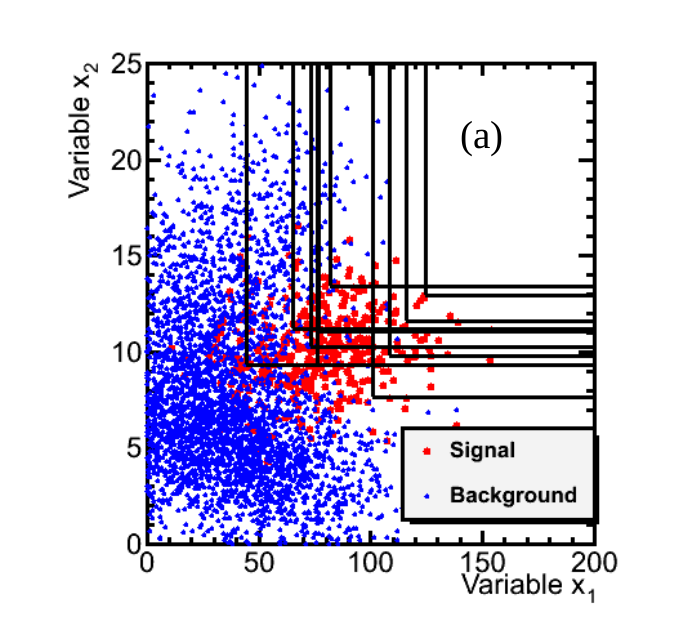
\includegraphics[width=0.85\textwidth]{figs/Grid_example.png}
	\caption{risultato grafico di un processo di taglio sulle due variabili $x_1$ e $x_2$ per la separazione del segnale dal background \cite{Metodi_multivariati}.}
	\label{fig:grid_example}
\end{figure}

La scelta della regione in cui fare il conteggio e' ottenuta grazie ad una ottimizzazione del rapporto segnale rumore al variare dei tagli. Questa ottimizzazione può essere ottenuta con molti metodi, di cui un esempio e' il Random Grid Search (RGS) che verrà presentato nella sezione \ref{iperparametri e grid search}. \\
In questo caso le selezioni sulle variabili $x_i$ sono fatte in modo indipendente, di conseguenza non si tiene conto di eventuali correlazioni tra le variabili e, se le distribuzioni di tali variabili per segnale e fondo sono molto simili, questo sistema può non essere molto efficiente.

\newpage
%%%%%%%%%%%%%%%%%%%%%%%%%%%%%%%%%%%%%%%%%%%%%%%%%%%%%%%%%%%%%%%
\subsection{Processi multivariati e analisi discriminante lineare}
\label{metodi lineari e discriminante di Fisher}

Nella sezione precedente è stato messo in evidenza il fatto che i sistemi di tagli non permettono di tener conto di eventuali correlazioni fra i dati.\\
Per poter tener conto delle correlazioni tra le variabili $x_i$ in esame, e poter sfruttare al meglio le variabili poco discriminanti e' possibile utilizzare delle selezioni ottenute grazie a selezioni su delle funzioni di un sottoinsieme delle variabili prese in esame. \\
Ogni volta che si considera una selezione fatta su una funzione di più di una variabile è possibile parlare di analisi multivariata e, per la ragione appena presentata, è necessario considerare i processi multivariati.\\
Il metodo di analisi multivariata più semplice e' quello del discriminante lineare, o discriminante di Fisher: si immagini di avere a disposizione un determinato set di eventi in input $\vec{x}_i$, ciascuno caratterizzato da un numero n di variabili (spazio n-dimensionale) e di volerli ripartire fra segnale e background.\\
Si definisce la funzione discriminante lineare nel seguente modo:
\begin{equation}
D(x_1 , x_2 , ... , x_n) = c_0 + c_1x_1 + ... +c_nx_n = c_0 + \sum_{i=0}^{n} c_ix_i 
\end{equation}
cioè una combinazione lineare delle componenti del vettore che rappresenta l'evento; il valore assunto dalla funzione per ogni singolo evento ne permette la separazione nelle due classi (nel presente caso segnale e background), utilizzando un valore di riferimento $D_0$. \\
A questo punto l'obiettivo è quello di massimizzare la distanza fra le due classi, ossia rendere massima la differenza dei valori assunti dalla funzione $D(\textbf{x})$ fra gli eventi appartenenti al background e quelli relativi al segnale. \\
Per ottenere una ottimizzazione del valore di selezione uno dei metodi più comuni è quello proposto da Fisher: si consideri un campione di eventi appartenenti al segnale e se ne definisca la media $\bm\mu_\textbf{s}$ e la deviazione standard $\sigma_s$ ed un campione appartenente al background, definendo anche qui la media $\bm\mu_\textbf{b}$ e la deviazione standard $\sigma_b$. A questo punto la migliore configurazione dei parametri è quella che massimizza la seguente funzione: 
\begin{equation}
F(\textbf{c}) = \frac{(\bm\mu_\textbf{s} - \bm\mu_\textbf{b})^2}{\sigma_s^2 + \sigma_b^2}
\end{equation} 
Il discriminante lineare e' il sistema multivariato con la forma funzionale più semplice. Si possono costruire discriminanti sempre più complessi nella forma funzionale.

 
%Dato che le componenti dei pattern possono essere tra loro correlate è possibile ridurre la dimensionalità dello spazio n-dimensionale da n a d (con d < n). Verrà posto un focus particolare sul problema della dimensionalità degli input della sezione \ref{curse_dim}, che servirà da trampolino di lancio per affrontare un metodo particolare del ML, il Variational Autoencoders. \\
%Come detto nella sezione precedente, i sistemi di tagli possono essere utilizzati per la separazione del segnale dal fondo ma hanno dei limiti piuttosto considerevoli che sono già stati illustrati. L'analisi discriminante è un metodo che permette di raggiungere lo stesso obiettivo di separazione, ma in modo più efficiente. \\
%L'analisi discriminante si definisce lineare quando la funzione classificatrice è, appunto, lineare. \\
%si immagini di avere a disposizione un determinato set di eventi in input $\vec{x}_i$, ciascuno caratterizzato da un numero n di variabili (spazio n-dimensionale) e di volerli ripartire fra segnale e background.\\
%Si definisce la funzione discriminante lineare nel seguente modo:
%\begin{equation}
%D(x_1 , x_2 , ... , x_n) = c_0 + c_1x_1 + ... +c_nx_n = c_0 + \sum_{i=0}^{n} c_ix_i 
%\end{equation}
%cioè una combinazione lineare delle componenti del vettore che rappresenta l'evento; il valore assunto dalla funzione per ogni singolo evento ne permette la separazione nelle due classi (nel presente caso segnale e background), utilizzando un valore di riferimento $D_0$. \\
%A questo punto l'obiettivo è quello di massimizzare la distanza fra le due classi, ossia rendere massima la differenza dei valori assunti dalla funzione $D(\textbf{x})$ fra gli eventi appartenenti al background e quelli relativi al segnale. \\
%Per ottenere una ottimizzazione del valore di selezione uno dei metodi più comuni è quello proposto da Fisher: si consideri un campione di eventi appartenenti al segnale e se ne definisca la media $\bm\mu_\textbf{s}$ e la deviazione standard $\sigma_s$ ed un campione appartenente al background, definendo anche qui la media $\bm\mu_\textbf{b}$ e la deviazione standard $\sigma_b$. A questo punto la migliore configurazione dei parametri è quella che massimizza la seguente funzione: 
%\begin{equation}
%F(\textbf{c}) = \frac{(\bm\mu_\textbf{s} - \bm\mu_\textbf{b})^2}{\sigma_s^2 + \sigma_b^2}
%\end{equation} 
%Il pregio di un'analisi di questo tipo è quello di non doversi necessariamente limitare a dei tagli paralleli agli assi. 

\color{red}
likelihood analysis ?? \\
commenti vuoti
\color{black}

\newpage
%%%%%%%%%%%%%%%%%%%%%%%%%%%%%%%%%%%%%%%%%%%%%%%%%%%%%%%%%%%%%%%%
\subsection{Machine Learning}
\label{ML}

Perché è utile il ML per l'obiettivo che è stato prefissato? Bisogna considerare il fatto che i sistemi multivariati descritti in sezione \ref{metodi lineari e discriminante di Fisher} dipendono fortemente dalla scelta dell'analista della funzione, o del metodo, da utilizzare per applicare la selezione del proprio campione. Il Machine Learning invece sfrutta algoritmi in grado di apprendere in maniera semi-autonoma la struttura dei campioni di background e segnale, ed è quindi in grado di stabilire quale sia il modo migliore per separare tali campioni. \\
L'approccio classico all'analisi dei dati prevede la disponibilità di un modello matematico, che dipende da una serie di parametri incogniti. Questi parametri vengono ricavati a partire dai dati sperimentali attraverso processi che possono essere sia analitici che numerici. \\
A differenza dei sistemi descritti fin ora, i sistemi di selezione autonoma non necessitano di un modello fisico-matematico su cui basare la propria selezione. \\
Bisogna distinguere tre macro-tipologie di approccio all'analisi dati nel machine learning:
\begin{itemize}
	
	\item APPRENDIMENTO SUPERVISIONATO \\
	In questa tipologia di apprendimento vengono presentati all'algoritmo degli input di esempio ed i relativi output desiderati, con lo scopo di apprendere una relazione generale che lega gli uni con gli altri; quindi per prima cosa si utilizza un campione di addestramento (\textit{training data set}), in cui l'algoritmo ottimizza la selezione per legare gli input agli output forniti in fase di addestramento. Una volta addestrato, l'algoritmo viene validato utilizzando un campione di test (\textit{test data set}) dove non vengono forniti gli output e se ne valuta l'efficienza di selezione;
	
	\item APPRENDIMENTO NON SUPERVISIONATO \\
	A differenza del caso supervisionato, nel training data set non sono presenti gli output attesi, quindi l'algoritmo deve essere in grado di apprendere autonomamente sia la struttura degli output desiderati, sia la miglior selezione per dividere i due campioni.
	Nel capitolo \ref{fisica_BSM_VAEs} verrà presentato un esempio di algoritmo non supervisionato per applicazioni nel campo della fisica delle particelle.
	
	\item APPRENDIMENTO PER RINFORZO \\
	Il $\textit{Reinforcement Learning}$ è basato sul concetto di ricompensa, cioè si permette all'algoritmo di esplorare un così detto ambiente e, in base all'azione compiuta, gli si fornisce un feedback positivo, negativo o indifferente. Un esempio classico prevede di voler addestrare un algoritmo per un particolare gioco: si farà in modo di fargli compiere una serie di partite in maniera iterativa e gli si assegnerà una ricompensa in caso di vittoria o una penalità in caso di sconfitta. \\ 
\end{itemize}

\newpage

Oltre al modo in cui gli algoritmi ottimizzano la selezione a partire dai loro campioni di addestramento, si deve distinguere anche il modo in cui vengono presentati i dati in uscita. In quest'ottica si possono individuare tre differenti tipologie di algoritmi:
\begin{itemize}
	
	\item CLASSIFICAZIONE \\
	Gli algoritmi di classificazione sono caratterizzati da un output discreto, cioè una serie di classi alle quali l'input può appartenere. Di solito questo metodo e' utilizzato da sistemi con apprendimento supervisionato. Un esempio di algoritmo di classificazione è quello che permette di distinguere se un particolare oggetto è presente o meno in un'immagine;
	
	\item REGRESSIONE \\
	La regressione è simile alla classificazione con la differenza che, in questo caso, l'output è continuo. Anche gli algoritmi di regressione sono adatti ad essere trattati con metodologie di apprendimento supervisionato;
	
	\item CLUSTERING \\
	Nel clustering l'obiettivo è sempre quello di dividere gli input in delle classi, tuttavia in questo caso tali classi non sono stabilite a priori. La natura di algoritmi di questo tipo li rende adatti ad essere trattati tramite metodi di apprendimento non supervisionato, proprio perché nel training data set gli eventi di input non sono etichettati (non è noto il relativo output) e quindi si richiede all'algoritmo di ricavare autonomamente le classi.
	
\end{itemize}

% nel machine learning non conosco la formo funzionale mentre nei metodi multivariati 
